\documentclass{oblivoir}
\usepackage{amsmath,amssymb,amsthm,kotex,mdframed,paralist}

\newcounter{num}
\newcommand{\prob}[1]
{\bigskip\noindent\refstepcounter{num}\textbf{문제 \arabic{num})#1}\par}

\newcommand{\ans}{
{\par\medskip\begin{mdframed}
\textbf{풀이 : }
\vspace{0.6\textheight}
\end{mdframed}\par
\raggedleft\textbf{답 : (\qquad\qquad\qquad\qquad\qquad\qquad)}
\par}\bigskip\bigskip}

\newcommand\ov[2]{\ensuremath{\overline{#1#2}}}

\newcommand\ve[2]{\ensuremath{\overrightarrow{#1#2}}}

%%%
\begin{document}
\title{혜령 05 - 벡터의 실수배}
\author{}
\date{\today}
\maketitle

%
\prob{}
\begin{figure}[h!]
\centering
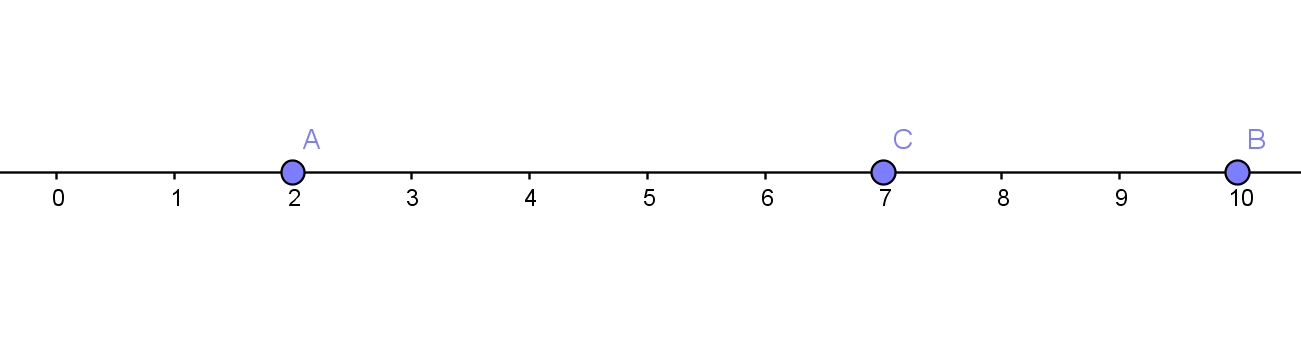
\includegraphics{01}
\end{figure}
\(\ve AC=k\ve AB\)를 만족하는 \(k\)의 값을 구하시오.

%
\prob{}
\begin{figure}[h!]
\centering
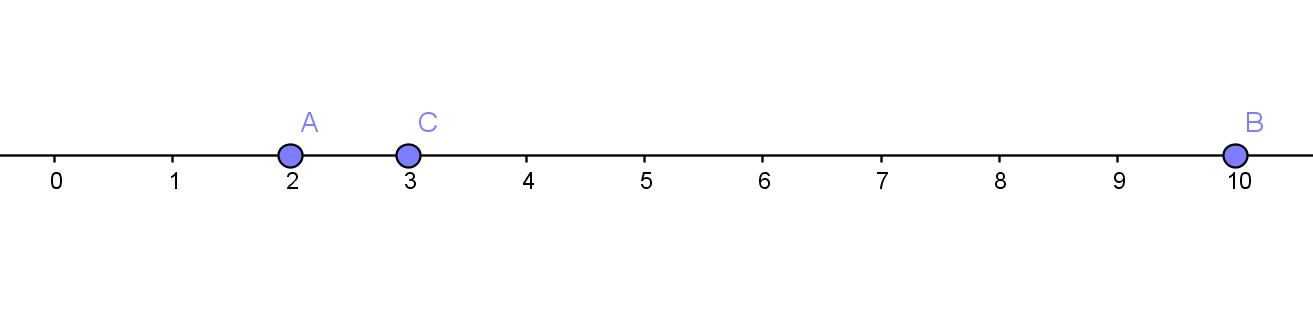
\includegraphics{02}
\end{figure}
\(\ve AC=k\ve AB\)를 만족하는 \(k\)의 값을 구하시오.

\newpage
%
\prob{}
\begin{figure}[h!]
\centering
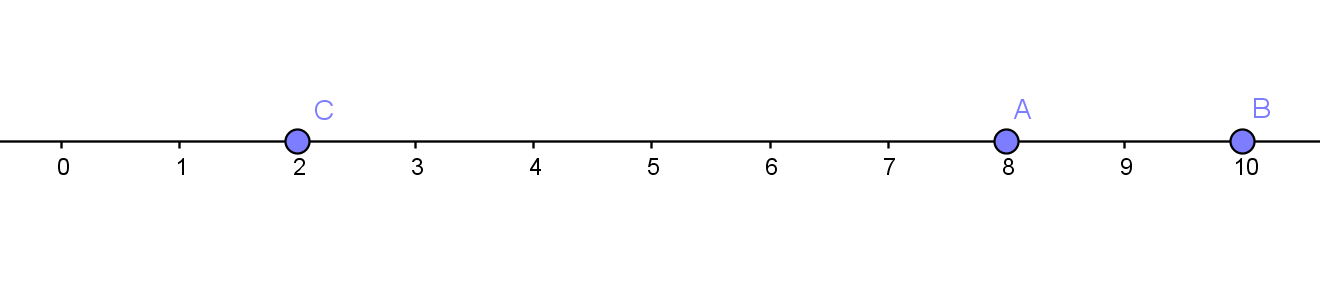
\includegraphics[width=0.9\textwidth]{03}
\end{figure}
\(\ve AC=k\ve AB\)를 만족하는 \(k\)의 값을 구하시오.

%
\prob{}
\begin{figure}[h!]
\centering
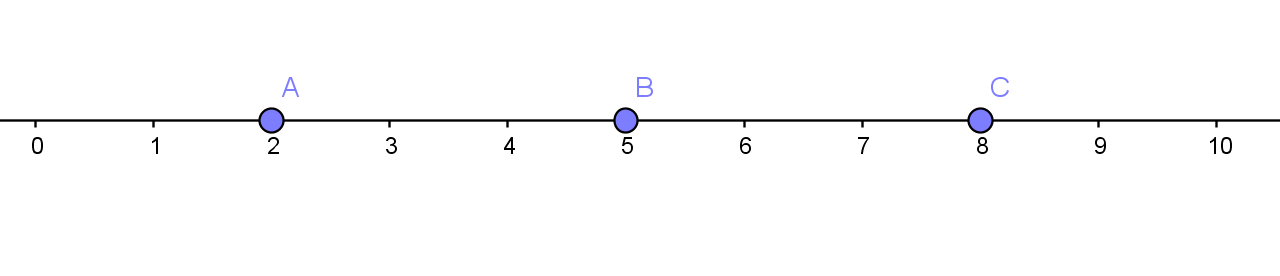
\includegraphics{04}
\end{figure}
\(\ve AC=k\ve AB\)를 만족하는 \(k\)의 값을 구하시오.

%
\prob{}
\begin{figure}[h!]
\centering
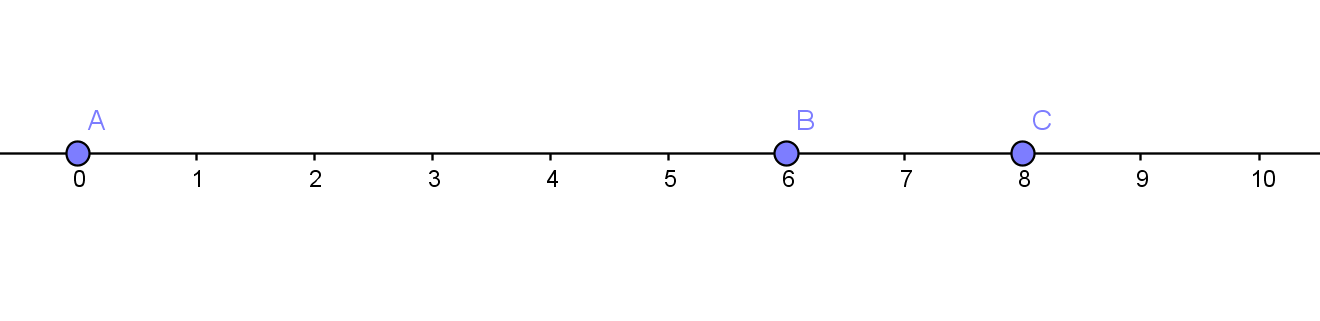
\includegraphics{05}
\end{figure}
\(\ve AC=k\ve AB\)를 만족하는 \(k\)의 값을 구하시오.

%
\prob{}
\begin{figure}[h!]
\centering
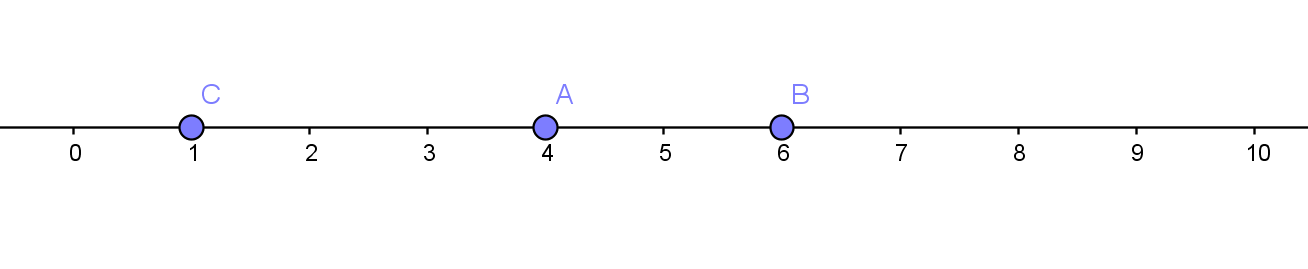
\includegraphics{06}
\end{figure}
\(\ve AC=k\ve AB\)를 만족하는 \(k\)의 값을 구하시오.

\newpage
%
\prob{}
다음 그림에서 \(C\)는 \(A\), \(B\)의 중점이고 \(D\)는 \(A\), \(B\)의 2:1 내분점이다.
\(\ve CD=k\ve AB\)를 만족하는 \(k\)의 값을 구하시오.
\begin{figure}[h!]
\centering
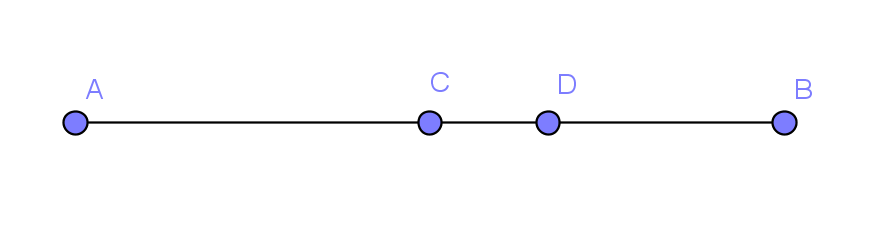
\includegraphics{07}
\end{figure}

%
\prob{}
다음 그림에서 \(C\)는 \(A\), \(B\)의 4:1 내분점이고 \(D\)는 \(A\), \(B\)의 1:2 내분점이다.
\(\ve CD=k\ve AB\)를 만족하는 \(k\)의 값을 구하시오.
\begin{figure}[h!]
\centering
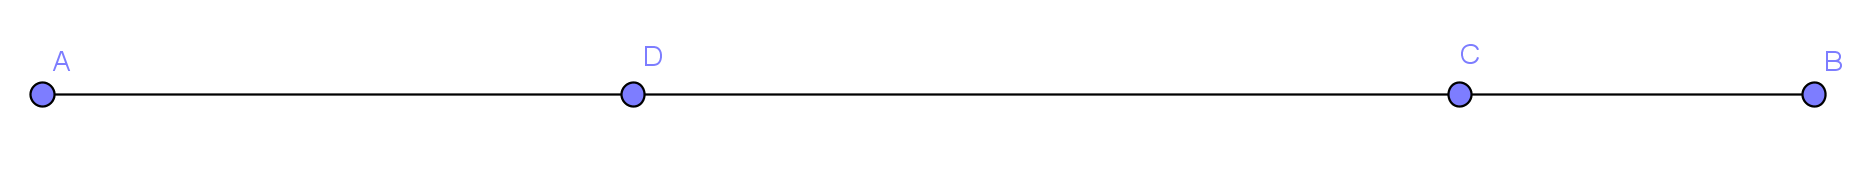
\includegraphics[width=0.9\textwidth]{08}
\end{figure}

%
\prob{}
\begin{figure}[h!]
\centering
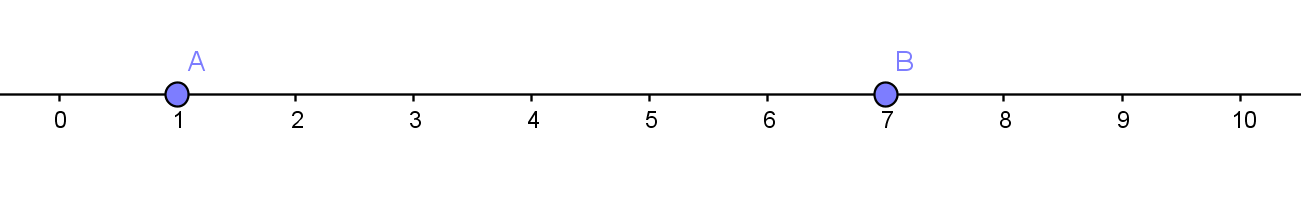
\includegraphics[width=0.9\textwidth]{09}
\end{figure}
다음 그림에서 \(\ve PA+2\ve PB=\vec{0}\)를 만족하는 \(P\)점의 좌표를 구하시오.

%
\prob{}
\begin{figure}[h!]
\centering
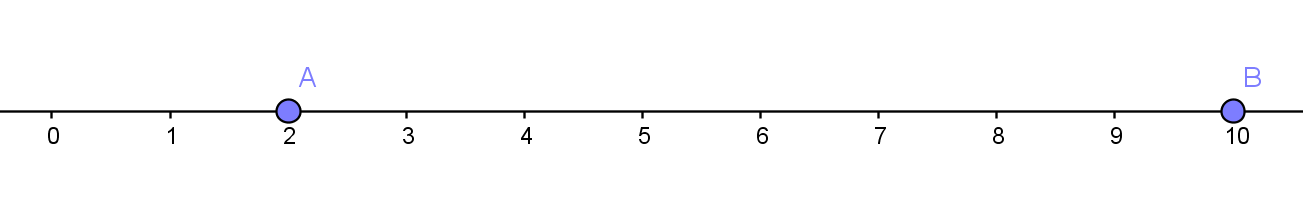
\includegraphics[width=0.9\textwidth]{10}
\end{figure}
다음 그림에서 \(3\ve PA+\ve PB=\vec{0}\)를 만족하는 \(P\)점의 좌표를 구하시오.

\newpage
%
\prob{}
\begin{figure}[h!]
\centering
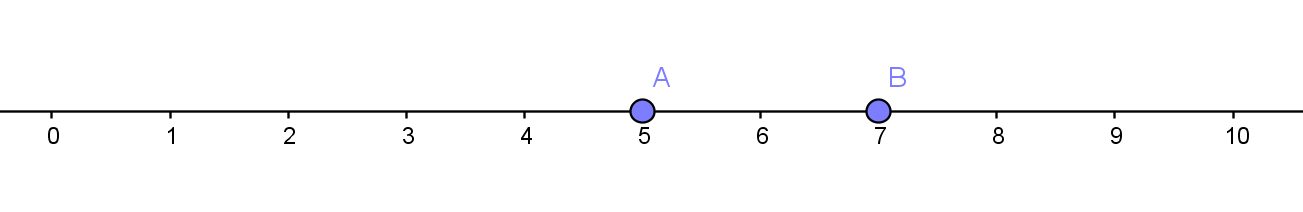
\includegraphics[width=0.9\textwidth]{11}
\end{figure}
다음 그림에서 \(\ve PA=2\ve PB\)를 만족하는 \(P\)점의 좌표를 구하시오.

%
\prob{}
\begin{figure}[h!]
\centering
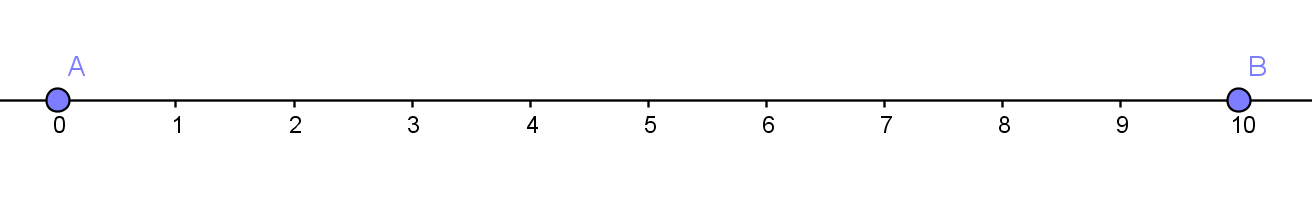
\includegraphics[width=0.9\textwidth]{12}
\end{figure}
다음 그림에서 \(\ve PB=-4\ve PA\)를 만족하는 \(P\)점의 좌표를 구하시오.

%
\prob{}
\begin{figure}[h!]
\centering
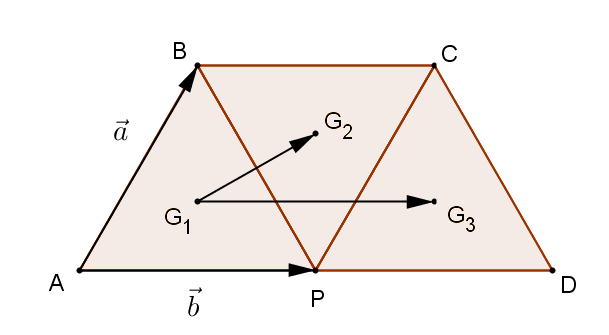
\includegraphics{13}
\end{figure}
정삼각형 \(PAB\), \(PBC\), \(PCD\)의 무게중심이 각각 \(G_1\), \(G_2\), \(G_3\)이다.
\(\ve AB=\vec a\), \(\ve AP=\vec b\)일 때, \(\ve {G_1}{G_2}=k\vec a+l\vec b\)와  \(\ve {G_1}{G_3}=m\vec a+n\vec b\)을 만족하는 실수 \(l\), \(m\), \(n\), \(k\)에 대해 \(l+m+n+k\)의 값을 구하시오.

\newpage
%%
%\prob{}
%\begin{figure}[h!]
%\centering
%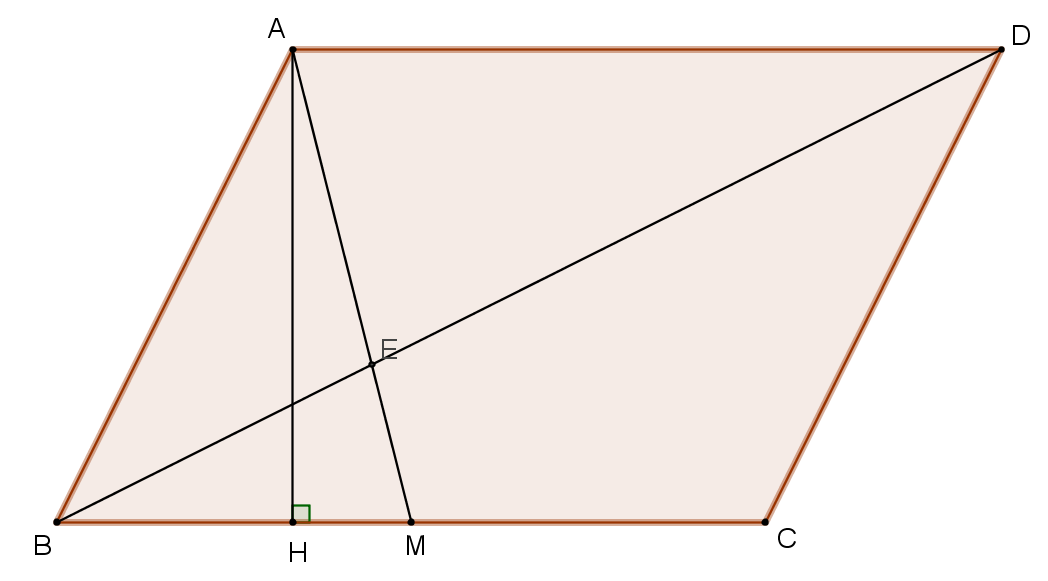
\includegraphics{14}
%\end{figure}
%평행사변형 \(ABCD\)에서 \(A\)에서 \(BC\)에 내린 수선의 발이 \(H\)이고, \(\ov AH=4\), \(\ov BH=2\) \(\ov BC=6\)이다.
%\(M\)이 \(BC\)의 중점이고, \(E\)는 \(\ov AM\)과 \(\ov BD\)의 교점일 때, \(\ve CE=a\ve BC+b\ve BA\)를 만족시키는 \(a\), \(b\)의 값을 구하시오.

%
\prob{}
\begin{figure}[h!]
\centering
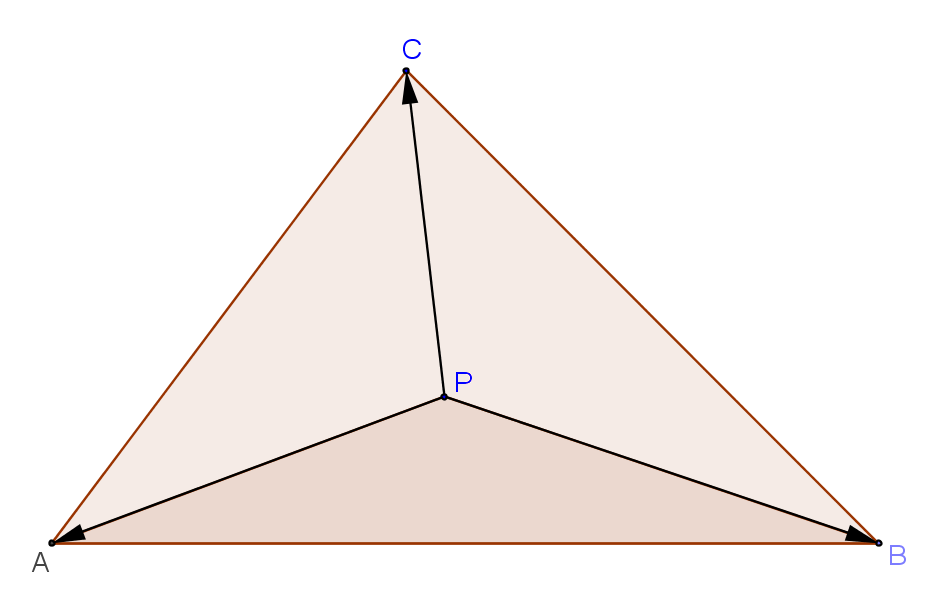
\includegraphics{15}
\end{figure}
\(\triangle ABC\)의 넓이는 \(60\)이다.
\(\ve PA+\ve PB+\ve PC=\vec 0\)을 만족하는 \(P\)에 대해 \(\triangle PAB\)의 넓이를 구하시오.

%
\prob{}
\begin{figure}[h!]
\centering
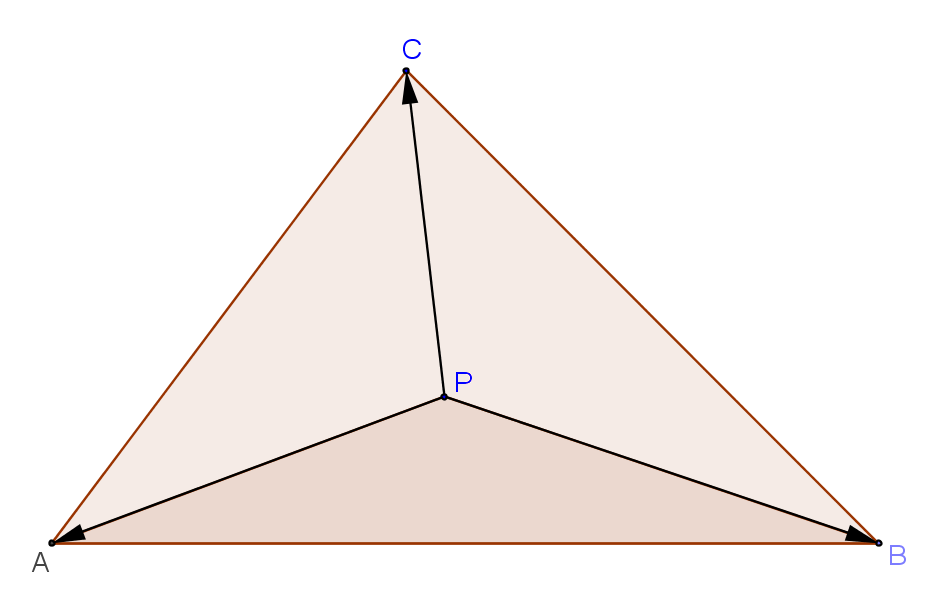
\includegraphics{15}
\end{figure}
\(\triangle ABC\)의 넓이는 \(60\)이다.
\(\ve PA+\ve PB+2\ve PC=\vec 0\)을 만족하는 \(P\)에 대해 \(\triangle PAB\)의 넓이를 구하시오.
\newpage

%
\prob{}
\begin{figure}[h!]
\centering
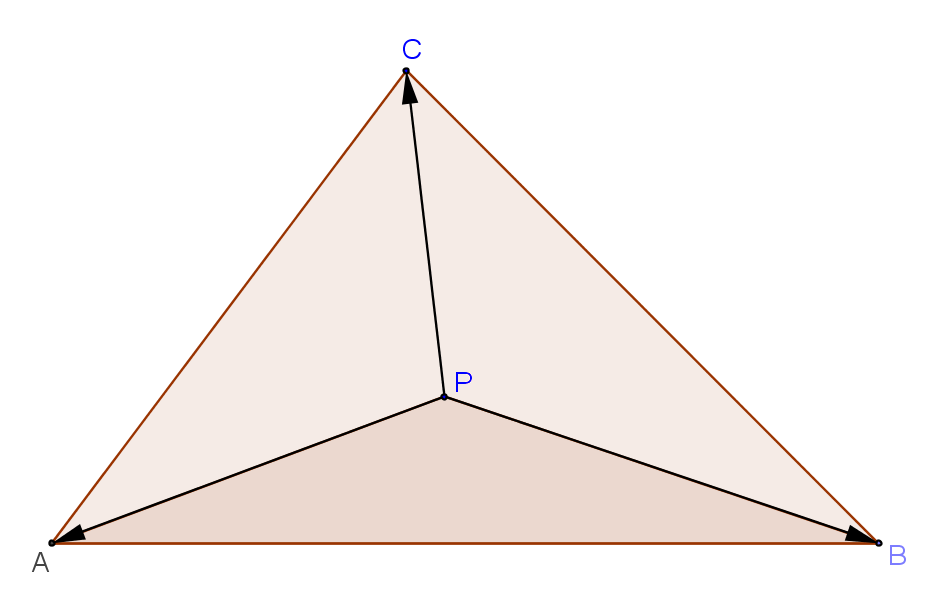
\includegraphics{15}
\end{figure}
\(\triangle ABC\)의 넓이는 \(60\)이다.
\(\ve PA+2\ve PB+3\ve PC=\vec 0\)을 만족하는 \(P\)에 대해 \(\triangle PAB\)의 넓이를 구하시오.

\end{document}